\documentclass{article}

\usepackage{fancyhdr}
\usepackage{extramarks}
\usepackage{amsmath}
\usepackage{amsthm}
\usepackage{amsfonts}
\usepackage{tikz}
\usepackage[plain]{algorithm}
\usepackage{algpseudocode}
\usepackage{xcolor}
\usepackage{enumitem}
\usepackage{amssymb}
\usepackage{todonotes}
\usepackage{mathtools}
\usepackage{wasysym}
\usepackage{cancel}
\usepackage{phaistos}
\usepackage[usestackEOL]{stackengine}[2013-10-15]
\def\x{\hspace{6ex}}    %BETWEEN TWO 1-DIGIT NUMBERS
\def\y{\hspace{4.9ex}}  %BETWEEN 1 AND 2 DIGIT NUMBERS
\def\z{\hspace{3.8ex}}    %BETWEEN TWO 2-DIGIT NUMBERS
\stackMath

\usetikzlibrary{automata,positioning}

%
% Basic Document Settings
%

\topmargin=-0.45in
\evensidemargin=0in
\oddsidemargin=0in
\textwidth=6.5in
\textheight=9.0in
\headsep=0.25in

\linespread{1.1}

\pagestyle{fancy}
\lhead{\hmwkAuthorName}
\chead{\hspace{2.5cm} \hmwkClass\ (\hmwkClassInstructor): \hmwkTitle}
\rhead{\firstxmark}
\lfoot{\lastxmark}
\cfoot{\thepage}

\renewcommand\headrulewidth{0.4pt}
\renewcommand\footrulewidth{0.4pt}

\setlength\parindent{0pt}

%
% Create Problem Sections
%

\newcommand{\enterProblemHeader}[1]{
    \nobreak\extramarks{}{Problem \arabic{#1} continued on next page\ldots}\nobreak{}
    \nobreak\extramarks{Problem \arabic{#1} (continued)}{Problem \arabic{#1} continued on next page\ldots}\nobreak{}
}

\newcommand{\exitProblemHeader}[1]{
    \nobreak\extramarks{Problem \arabic{#1}}{Problem \arabic{#1} continued on next page\ldots}\nobreak{}
    \stepcounter{#1}
    \nobreak\extramarks{Problem \arabic{#1}}{}\nobreak{}
}

\newcount\colveccount
\newcommand*\colvec[1]{
        \global\colveccount#1
        \begin{pmatrix}
        \colvecnext
}
\def\colvecnext#1{
        #1
        \global\advance\colveccount-1
        \ifnum\colveccount>0
                \\
                \expandafter\colvecnext
        \else
                \end{pmatrix}
        \fi
}

\setcounter{secnumdepth}{0}
\newcounter{partCounter}
\newcounter{homeworkProblemCounter}
\setcounter{homeworkProblemCounter}{1}
\nobreak\extramarks{Problem \arabic{homeworkProblemCounter}}{}\nobreak{}

%
% Homework Problem Environment
%
% This environment takes an optional argument. When given, it will adjust the
% problem counter. This is useful for when the problems given for your
% assignment aren't sequential. See the last 3 problems of this template for an
% example.
%
\newenvironment{homeworkProblem}[1][-1]{
    \ifnum#1>0
        \setcounter{homeworkProblemCounter}{#1}
    \fi
    \section{Problem \arabic{homeworkProblemCounter}}
    \setcounter{partCounter}{1}
    \enterProblemHeader{homeworkProblemCounter}
}{
    \exitProblemHeader{homeworkProblemCounter}
}

%
% Homework Details
%   - Title
%   - Due date
%   - Class
%   - Section/Time
%   - Instructor
%   - Author
%

\newcommand{\hmwkTitle}{Assignment 6}
\newcommand{\hmwkDueDate}{1 December, 2018}
\newcommand{\hmwkClass}{Probability \& Statistics}
\newcommand{\hmwkClassTime}{Fall Semester}
\newcommand{\hmwkClassInstructor}{Prof. D. Eynard}
\newcommand{\hmwkAuthorName}{\textbf{A. Romanelli} / \textbf{A. Vicini}}

%
% Title Page
%

\title{
    \vspace{2in}
    \textmd{\textbf{\hmwkClass:\ \hmwkTitle}}\\
    \normalsize\vspace{0.1in}\small{Due\ on\ \hmwkDueDate\ at 8:30am}\\
    \vspace{0.1in}\large{\textit{\hmwkClassInstructor}}
    \vspace{3in}
}

\author{\hmwkAuthorName}
\date{}

\renewcommand{\part}[1]{\textbf{\large Part \Alph{partCounter}}\stepcounter{partCounter}\\}

%
% Various Helper Commands
%

% Useful for algorithms
\newcommand{\alg}[1]{\textsc{\bfseries \footnotesize #1}}

% For derivatives
\newcommand{\deriv}[1]{\frac{\mathrm{d}}{\mathrm{d}x} (#1)}

% For partial derivatives
\newcommand{\pderiv}[2]{\frac{\partial}{\partial #1} (#2)}

% Integral dx
\newcommand{\dx}{\mathrm{d}x}

% Alias for the Solution section header
\newcommand{\solution}{\textbf{\large Solution}}

% Probability commands: Expectation, Variance, Covariance, Bias
\newcommand{\E}{\mathrm{E}}
\newcommand{\Var}{\mathrm{Var}}
\newcommand{\Cov}{\mathrm{Cov}}
\newcommand{\Bias}{\mathrm{Bias}}

\begin{document}

\maketitle

\pagebreak

\begin{homeworkProblem}
	\begin{enumerate}[label=\textbf{\alph*)}]
		\item In order to find $P(X > 22.07)$ we need to find the corresponding value in the $\Phi$ distribution, that is, we need to normalise the considered value:
		$$
			P(X > 22.07) = P\left(X^* > \frac{22.07-\mu}{\sigma}\right)
		$$
		Knowing that $\Var(X) = \sigma^2 = 0.16$, we can write:
		$$
			P\left(X^* > \frac{22.07 - 21.37}{0.4}\right)
		$$
		$$
			P\left(X^* > \frac{0.7}{0.4}\right) = P\left(X^* > 1.75\right)
		$$
		Since this last inequality is about the normalised random variable $X^*$ we can look up the cumulative probability for $X^* < 1.75$ and subtract it from the total probability to get its complement, which is what we are looking for.
		$$
			\Phi(1.75) = 0.9599
		$$
		$$
			P(X^* > 1.75) = 1 - \Phi(1.75) = 1 - 0.9599 = 0.0401 \approx 4\%
		$$
		\item We know want to compute $P(Y \leq 2)$, which is the probability that out of 15 mints, at most 2 weigh more than 20.857g. This means that we are dealing with a binomial distribution, since a mint can only weigh less or more. But what is the probability of such events?
		\\ \\ 
		We need to compute then $P(X < 20.857)$, by normalising again we get:
		$$
			P\left(X^* < \frac{20.857 - 21.37}{0.4}\right) = P\left(X^* < \frac{-0.513}{0.4}\right) = P(X^* < -1.2825) = \Phi(-1.2825) \approx 0.1003 \approx 10\%
		$$
		Thus we can now compute our probability as a binomial distribution:
		$$P(k) = \sum_{i = 0}^k {n \choose i}p^i(1-p)^{n-i}$$
		$$P(2) = {15 \choose 0}(0.9)^{15} + {15 \choose 1}(0.1)(0.9)^{14}+ {15 \choose 2}(0.001)(0.9)^{13} \approx 0.8159 \approx 82\%$$
	\end{enumerate}
\end{homeworkProblem}
\newpage
\begin{homeworkProblem}
	\begin{enumerate}[label=\textbf{\alph*)}]
		\item If we want to find $\sigma$ of a known distribution $N(\mu=12.1, \sigma^2)$ in order for $P(X < 12) = 0.01$ to be true. Thus we want to find for which value of $\Phi$ must coincide to the same value.
		$$
			P\left(X^* < \frac{12-12.1}{\sigma}\right) = 0.01
		$$
		By looking at the table of the standard normal CDF $\Phi(z)$, we can see that: 
		$$
			\Phi(-2.33) = 0.01
		$$
		Which implies:
		$$
			\frac{-0.1}{\sigma} = -2.33
		$$$$
			\sigma = \frac{0.1}{2.33} \approx 0.043
		$$
		\item Just like we did before, we can derive $\mu$ by fixing $\sigma = 0.05$ so that $P(X < 12) = 0.01$:
		$$
			\frac{12 - \mu}{0.05} = -2.33
		$$$$
			12 - \mu = -\frac{2.33}{20} 
		$$$$
			\mu = 12.1165
		$$
	\end{enumerate}
\end{homeworkProblem}
\newpage
\begin{homeworkProblem}
	The times required to produce an item are independent random variables between 1 and 5 with the same probability:
	\begin{figure}[h]
		\centering
		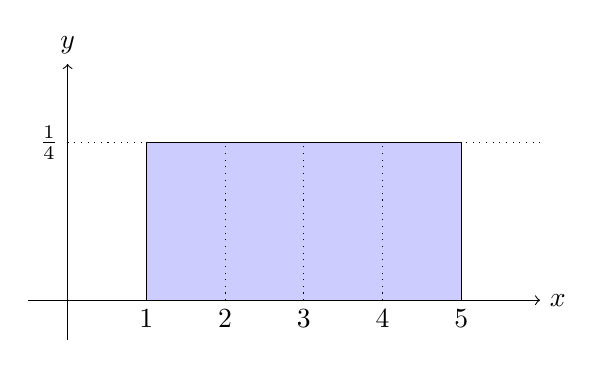
\begin{tikzpicture}
			\draw[dotted] (0,2) node[left] {$\frac14$} -- (6,2);
			\node[below] at (1,0) {$1$};
			\node[below] at (2,0) {$2$};
			\node[below] at (3,0) {$3$};
			\node[below] at (4,0) {$4$};
			\node[below] at (5,0) {$5$};
			\fill[color=blue!20!white, draw=black] (1,0) rectangle (5,2);
			\draw[dotted] (2,0) -- (2,2);
			\draw[dotted] (3,0) -- (3,2);
			\draw[dotted] (4,0) -- (4,2);
			\draw[->] (-0.5,0) -- (6,0) node[right] {$x$};
			\draw[->] (0,-0.5) -- (0,3) node[above] {$y$};
%	      \draw[scale=0.5,domain=-3:3,smooth,variable=\x,blue] plot ({\x},{\x*\x});
%	      \draw[scale=0.5,domain=-3:3,smooth,variable=\y,red]  plot ({\y*\y},{\y});
	    \end{tikzpicture}
	    \caption{Uniform distribution: $p(x)= \frac14, \quad x\in \{1, \dots, 5\}$}
	\end{figure}\\
	We can thus compute the mean $\mu$, that is the average time for a single piece:
	$$\E[X] = \int_{1}^{5}{\frac14 x\ dx} = \frac14 \int_1^5x\ dx= \frac14 \left[\frac12 x^2\right]_1^5 = \frac14 \left[\frac{25}2 - \frac12\right] = \frac{12}4 = 3$$
	$$\mu = 3$$
	We now want to compute $\Var(X)$:
	$$\Var(X) = \E[X^2] - \E[X]^2$$
	$$\E[X^2] = \frac14\int_1^5 x^2\ dx = \frac14\left[\frac13 x^3\right]_1^5 = \frac14 \left[\frac{125}3 - \frac13\right] = \frac{124}{12} = \frac{31}3 $$
	$$\Var(X) = \frac{31}3 - 3^2 = \frac{31}3 - \frac{27}3 = \frac43$$
	$$\Var(X) = \sigma^2 = \frac43$$
	$$\sigma = \sqrt{\frac43} = \frac2{\sqrt3}$$
	We should know define a new random variable $S_n$ which is associated to the sum of the times for $n$ different items being produced:
	$$S_n = X_1 + \dots + X_n = \sum_{i=1}^n X_i, \quad 0 < i \leqslant n$$
	$$\E[S_n] = n \cdot \E[X_i] = 3n = \mu$$
	$$\Var(S_n) = n \cdot \Var(X_i) = \frac43n$$
	$$\sigma = \sqrt{\Var(S_n)} = 2\sqrt{\frac n3}$$
	Now that we have a normal distribution for a random variable $S_n$, we go back to our original question and to our hint that:
	$$P(N_{320} \geq 100) = P(S_{100} < 320)$$
	Where $S_{100}$ is exactly our random variable $S_n$ with $n=100$. \\
	Let us normalise the right side of this equation and substitute in:
	$$P\left(S_n^* \leq \frac{320 - \mu}{\sigma}\right) = P\left(S_n^* \leq \frac{320 - 3n}{2\sqrt{\frac n3}}\right) $$
	$$
		P\left(S_n^* \leq \frac{320 - 300}{\frac{20}{\sqrt3}}\right)  = P\left(S_n^* \leq \frac{1}{\frac{1}{\sqrt3}}\right) = P\left(S_n^* \leq \sqrt3\right) = \Phi(\sqrt3) \approx 0.9582 \approx 96\%
	$$
\end{homeworkProblem}
\newpage
\begin{homeworkProblem}
	We'll use the Bell-curve approximation to give bound to the binomial distribution for the Casino games. \\
	Just like we did for the previous assignment, we can define again the variable $X_n = \frac1n\sum_{i=1}^n X_i$, with the already known $\mu = \frac12, \sigma^2 = \frac1{4n} $ \\\\
	The next step will consist in normalising the current distribution of $X_n$ into the standard normal distribution $X_n^*$:
	$$
		X_n^* = \frac{X_n - \mu}{\sigma}
	$$
	\begin{enumerate}[label=\textbf{\alph*)}]
		\item With $n = 40$ and $p = 0.7$: \\
		This means that $\sigma = \sqrt{\frac1{4n}} = \frac1{2\sqrt{n}} = \frac1{2\sqrt{40}} = 0.079$ and that $\epsilon = p - \E[X_n] = p - \mu = 0.7 - 0.5 = 0.2$ \\ \\ 
		$$1 - \Phi\left(\frac{\frac15}{\frac1{\sqrt{160}}}\right) = 1 - \Phi\left(\frac{4\sqrt{10}}5\right) \approx 1 - \Phi(2.53) \approx 1 - 0.9943 = 0.0057 $$
		\item Given $n = 40, p = 0.501$: \\
		Consequently, we get: $\sigma$ stays the same and $\epsilon = 0.501 - 0.5 = 0.001$
		$$1 - \Phi\left(\frac{\frac1{100}}{\frac1{\sqrt{160}}}\right) = 1 - \Phi\left(\frac{\sqrt{10}}{25}\right) = 1 - \Phi(0.01) \approx 1 - 0.5040 = 0.496$$
		\item Given $n = 1500$ and $p = 0.6$ we get $\sigma = \frac1{2\sqrt{1500}} = 0.013, \epsilon = p - \E[X_n] = 0.6 - 0.5 = 0.1$
		$$1 - \Phi\left(\frac{\frac1{10}}{\frac1{20\sqrt{15}}}\right) = 1 - \Phi\left(\frac{20\sqrt{15}}{10}\right) = 1 - \Phi(2\sqrt{15}) \approx 0$$
		\item Given $n = 1500$ and $p = 0.501$ we get the same $\sigma$ and $\epsilon = 0.501 - 0.5 = 0.001$
		$$
			1 - \Phi\left(\frac{20\sqrt{15}}{1000}\right) = 1 - \Phi\left(\frac{\sqrt{15}}{50}\right) \approx 1 - 0.530871 = 0.469129
		$$
		\item Given $n = 1000000, p = 0.7$ we get $\sigma = \frac1{2\cdot 1000}, \epsilon = 0.7 - 0.5 = 0.2$
		$$
			1 - \Phi\left(\frac{2000}{5}\right) = 1 - \Phi(400) \approx 0
		$$
		\item Given $n = 1000000, p = 0.501$ thus we have the same $\sigma$ and $\epsilon = 0.001$
		$$
			1 - \Phi\left(\frac{\frac1{1000}}{\frac{1}{2000}}\right) = 1 - \Phi\left(\frac{2000}{1000}\right) = 1 - \Phi(2) \approx 1 - 0.97725 = 0.02275
		$$
	\end{enumerate}
	For all of the previous points, the Chebyshev inequality was always respected and always provided a valid upper bound.

\end{homeworkProblem}
\end{document}
